%===================================================================================
% Chapter: Metodologia
%===================================================================================
\chapter{Experimentación y Resultados}\label{chapter:resultados}
%\addcontentsline{toc}{chapter}{Marco Teórico}
%===================================================================================

En este capítulo bla bla

\section{Datos para la Validación del Modelo}
En el presente trabajo los datos provienen del Estudio en Lactantes Fase I/II para PCV7-TT (Instituto Finlay de Vacunas, 2019), cuyo principal objetivo era caracterizar la seguridad de VCN7-T y evaluar la no inferioridad de VCN7-T con respecto a Prevnar13® administrados en esquemas concomitante con las vacunas Va-Mengoc- BC® y Heberpenta® incluyendo lactantes de 2 a 3 meses de edad.

Se cuenta con datos de 240 sujetos divididos en dos grupos:
\begin{enumerate}
    \item Vacunados con VCN7-T
    \item Vacunados con Prevnar13®
\end{enumerate}

Para la validación del modelo nos centraremos en el grupo de sujetos vacunados con VCN7-T

\subsection{Limpieza de Datos}
Antes de trabajar con los datos fue requerido un proceso de limpieza de los mismos. 


\subsubsection{Datos Faltantes}
Las gráficas siguientes muestran la cantidad de valores, por columna del \textit{dataset} que son nulas o vacías. 
\begin{figure}[h]
    \centering
    % Primera fila
    \begin{minipage}{0.45\textwidth}
        \centering
        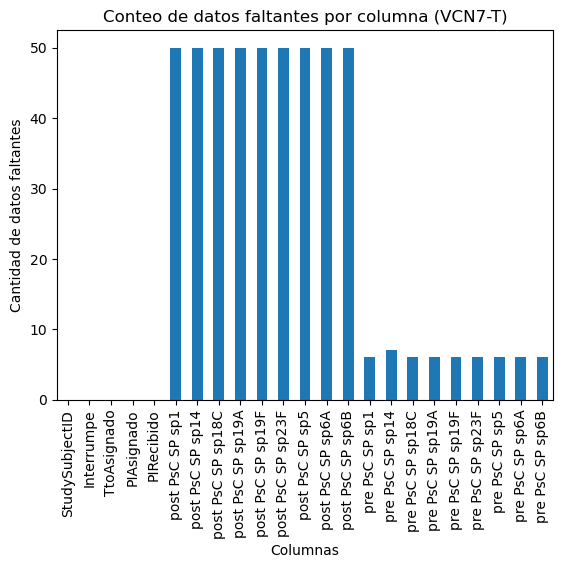
\includegraphics[width=1.0\textwidth]{Graphics/mdq.png}
        \caption{}
        \label{fig:mdq}
    \end{minipage}%
    \hfill
    \begin{minipage}{0.45\textwidth}
        \centering
        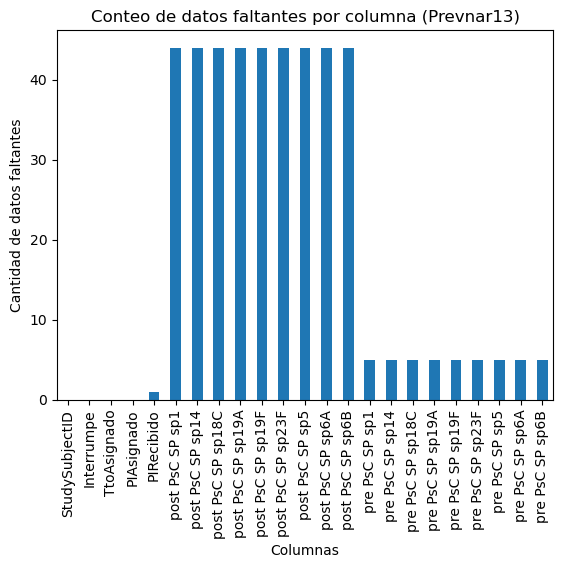
\includegraphics[width=1.0\textwidth]{Graphics/mdp.png}
        \caption{}
        \label{fig:mdp}
    \end{minipage}

\end{figure}



Los altos valores en las columnas 'post PsC SP [serotipo]' se deben a que el estudio utiliza dos esquemas de vacunación.
\begin{itemize}
    \item esquema (2p + 1): 
    \item esquema (3p + 0):
\end{itemize}
Se puede asumir que los sujetos con valores nulos en las columnas 'post PsC SP [serotipo]' fueron vacunados siguiendo un esquema (3p + 0), sin embargo para la validación del modelo nos centramos en los sujetos vacunados siguiendo el esquema (2p + 1).

\subsubsection{Valores inconsistentes}
Durante el análisis de los datos, se detectaron valores atípicos con magnitudes aparentemente inconsistentes. Una inspección minuciosa reveló que dichos valores correspondían a cifras significativas expresadas con distinta notación decimal; en particular, mientras la mayoría de los datos estaban representados con tres cifras significativas correctamente posicionadas, algunos carecían del punto decimal, lo que implicaba una escala incorrecta. Para homogeneizar la representación, se aplicó una corrección consistente en dividir por 1000 los valores afectados. Esta normalización facilitó una presentación más coherente y uniforme de los datos.

\vspace{0.5cm}

\textbf{Gráficas de valores pre-refuerzo(post vacunación primaria) contra valores post-refuerzo}

\begin{figure}[h]
    \centering
    % Primera fila
    \begin{minipage}{0.45\textwidth}
        \centering
        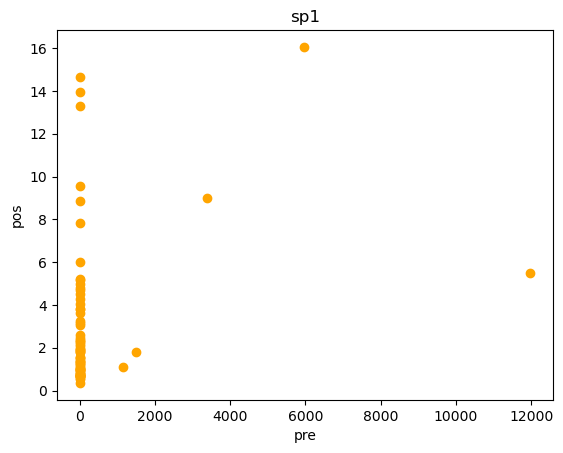
\includegraphics[width=\linewidth]{Graphics/sp1d.png}
        \caption{Serotipo 1 antes de la corrección}
        \label{fig:sp1d}
    \end{minipage}%
    \hfill
    \begin{minipage}{0.45\textwidth}
        \centering
        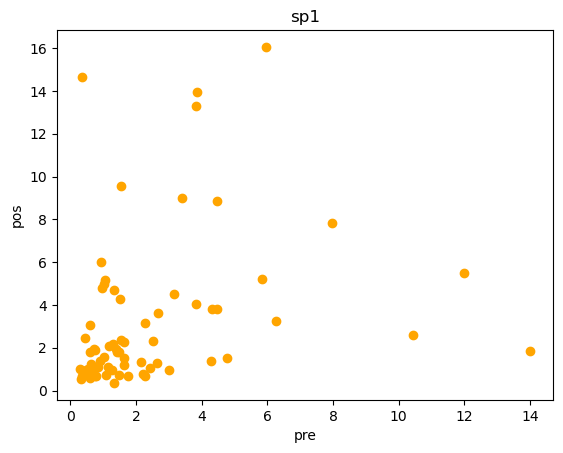
\includegraphics[width=\linewidth]{Graphics/sp1.png}
        \caption{Serotipo 1 después de la corrección}
        \label{fig:sp1}
    \end{minipage}

\end{figure}

\begin{figure}[H]
    \begin{minipage}{0.45\textwidth}
        \centering
        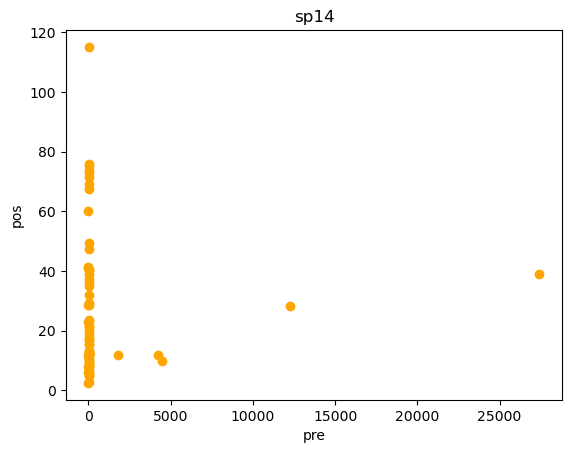
\includegraphics[width=\linewidth]{Graphics/sp14d.png}
        \caption{Serotipo 14 antes de la corrección}
        \label{fig:sp14d}
    \end{minipage}%
    \hfill
    \begin{minipage}{0.45\textwidth}
        \centering
        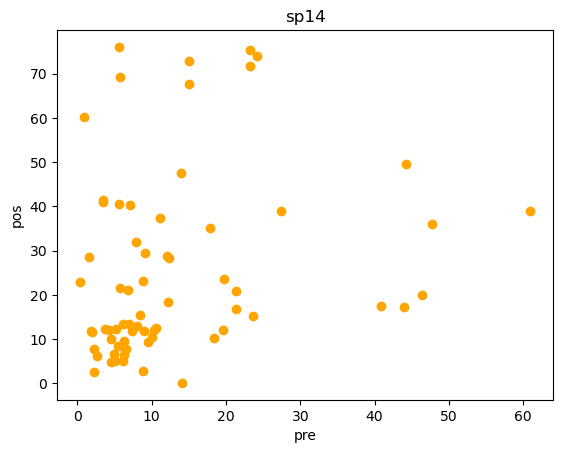
\includegraphics[width=\linewidth]{Graphics/sp14.png}
        \caption{Serotipo 14 después de la corrección}
        \label{fig:sp14}
    \end{minipage}
\end{figure}


\section{Entrenamiento}
Para el entrenamiento del modelo se tomó el 70\% de los datos. este proceso tiene como objetivo estimar los parámetros \texttt{plasma\_production\_factor} y \texttt{memory\_production\_factor}

\subsection{Exploración del espacio de parámetros}

Para explorar el espacio de parámetros durante el proceso de entrenamiento se utilizó la metaheurística de Recocido Simulado (\textit{Simulated Annealing}), un algoritmo inspirado en el proceso físico de enfriamiento de materiales. Este método permite realizar una búsqueda estocástica eficiente que evita quedar atrapado en óptimos locales, gracias a su capacidad para aceptar temporalmente soluciones peores con una probabilidad controlada por un parámetro denominado temperatura.

El algoritmo comienza con una temperatura inicial alta que permite explorar ampliamente el espacio de soluciones, aceptando cambios incluso si empeoran la función objetivo. A medida que avanza el proceso, la temperatura decrece siguiendo un protocolo de enfriamiento cuidadosamente diseñado, reduciendo gradualmente la probabilidad de aceptar soluciones peores y enfocando la búsqueda en regiones de baja energía o costo.

% Esta estrategia facilita la convergencia hacia un mínimo global o soluciones cercanas, especialmente en problemas con múltiples óptimos locales o funciones objetivo complejas y no continuas. La implementación del Recocido Simulado en nuestro entrenamiento incluyó la definición de parámetros clave como la temperatura inicial y final, la tasa y el método de enfriamiento, así como criterios de convergencia basados en el número de iteraciones y la estabilidad de las soluciones encontradas.


\subsection{Métrica de Optimización}

La métrica utilizada como función objetivo durante el entrenamiento del modelo es la \textit{distancia de Chamfer}, una medida que cuantifica la similitud entre dos conjuntos de puntos en el espacio. Esta métrica es especialmente adecuada para comparar nubes de puntos, ya que evalúa la proximidad bidireccional entre cada punto de un conjunto y su vecino más cercano en el otro conjunto, capturando así diferencias en forma y distribución.

El cálculo de la distancia de Chamfer se realiza en dos pasos principales:

\begin{enumerate}
    \item Para cada punto en el primer conjunto, se encuentra el punto más cercano en el segundo conjunto y se calcula la distancia euclidiana entre ellos. Se obtiene el promedio de estas distancias.
    \item Se repite el procedimiento invirtiendo los roles de los conjuntos, es decir, desde el segundo conjunto hacia el primero.
\end{enumerate}

Finalmente, la distancia de Chamfer se define como la suma (o promedio) de estos dos valores, formalmente expresada como:

\[
D_{\mathrm{Chamfer}}(S_1, S_2) = \frac{1}{|S_1|} \sum_{x \in S_1} \min_{y \in S_2} \|x - y\|_2 \;+\; \frac{1}{|S_2|} \sum_{y \in S_2} \min_{x \in S_1} \|y - x\|_2
\]

donde \( S_1 \) y \( S_2 \) son los conjuntos de puntos simulados y reales, respectivamente, y \(\|\cdot\|_2\) denota la distancia euclidiana.

Esta métrica es relevante porque permite evaluar de forma robusta la similitud geométrica entre las salidas simuladas del modelo y los datos reales, incluso cuando los puntos no están emparejados uno a uno. Minimizar la distancia de Chamfer durante el entrenamiento guía al modelo a generar salidas que se ajusten estrechamente a la distribución y forma de los datos observados.


\section{Validación}
Para el proceso de validación se tomó el 30\% restante de los datos y se generó una conjunto de la misma cantidad de puntos con los parámetros obtenidos del proceso de entrenamiento y se calculó la distancia Chamfer para estos conjuntos. Los resultados obtenidos se muestran a continuación:

\begin{table}[h]
\centering
\caption{Distancia de Chamfer por Serotipo}
\begin{tabular}{|c|c|}
\hline
\textbf{Serotipo} & \textbf{Distancia Chamfer} \\
\hline
1   & 3.422  \\
14  & 26.348 \\
18C & 2.773  \\
19F & 4.443  \\
23F & 4.803  \\
5   & 3.241  \\
6B  & 8.539  \\
\hline
\end{tabular}
\label{tab:chamfer_serotipos}
\end{table}

\textbf{Gráficas de valores pre-refuerzo(post vacunación primaria) contra valores post-refuerzo}
\begin{itemize}
    \item Puntos naranjas: datos de validación.
    \item Puntos azules: salida del modelo.
\end{itemize}
\begin{figure}[h]
    \centering
    % Primera fila
    \begin{minipage}{0.45\textwidth}
        \centering
        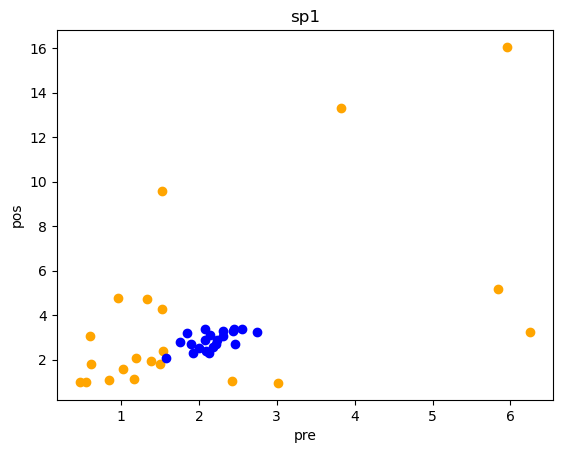
\includegraphics[width=\linewidth]{Graphics/sp1t.png}
        \caption{Serotipo 1}
        \label{fig:sp1t}
    \end{minipage}%
    \hfill
    \begin{minipage}{0.45\textwidth}
        \centering
        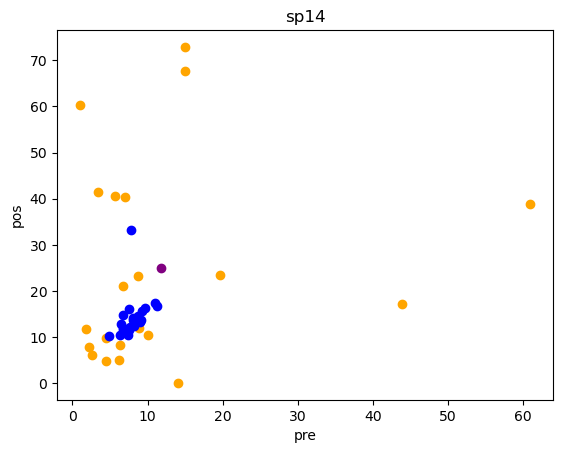
\includegraphics[width=\linewidth]{Graphics/sp14t.png}
        \caption{Serotipo 14}
        \label{fig:sp14t}
    \end{minipage}
\end{figure}
\begin{figure}
    
    \begin{minipage}{0.45\textwidth}
        \centering
        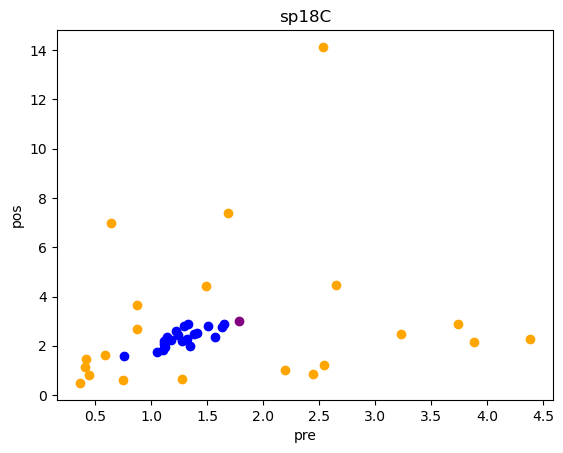
\includegraphics[width=\linewidth]{Graphics/sp18ct.png}
        \caption{Serotipo 18C}
        \label{fig:sp18ct}
    \end{minipage}
    \begin{minipage}{0.45\textwidth}
        \centering
        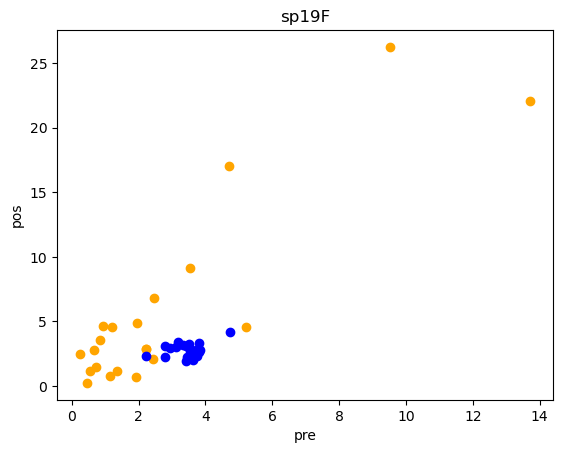
\includegraphics[width=\linewidth]{Graphics/sp19ft.png}
        \caption{Serotipo 19F}
        \label{fig:sp19ft}
    \end{minipage}
\end{figure}
\begin{figure}
    \begin{minipage}{0.45\textwidth}
        \centering
        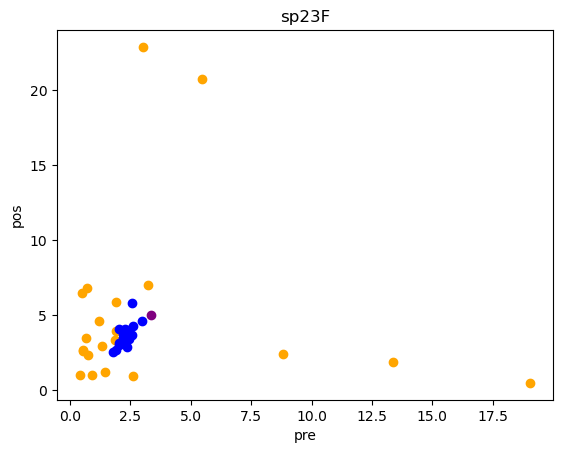
\includegraphics[width=\linewidth]{Graphics/sp23ft.png}
        \caption{Serotipo 23F}
        \label{fig:sp23ft}
    \end{minipage}
    \begin{minipage}{0.45\textwidth}
        \centering
        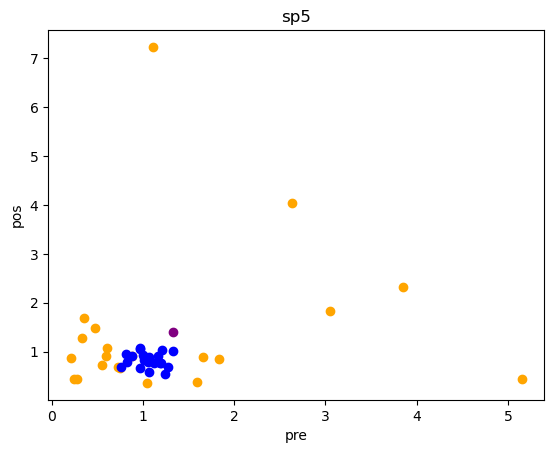
\includegraphics[width=\linewidth]{Graphics/sp5t.png}
        \caption{Serotipo 5}
        \label{fig:sp5t}
    \end{minipage}
\end{figure}
\begin{figure}
    \begin{minipage}{0.45\textwidth}
        \centering
        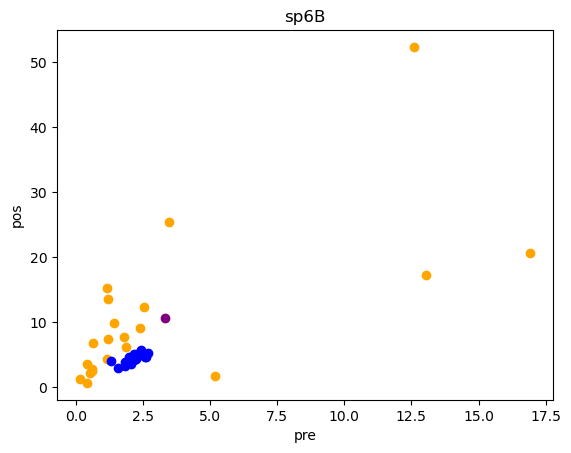
\includegraphics[width=\linewidth]{Graphics/sp6bt.png}
        \caption{Serotipo 6B}
        \label{fig:sp6bt}
    \end{minipage}

\end{figure}